\documentclass[twoside,11pt,ShortChapTitles]{BYUTextbook}

\usepackage{soul}
\renewcommand{\vec}[1]{\ensuremath{\mathbf{#1}}}
\usepackage{siunitx}
\sisetup{round-mode = figures,
  round-precision = 3, scientific-notation=true}
  \usepackage{marginfix}

\usepackage{mathtools}






\setcounter{chapter}{4}

\begin{document}
\chapter{Experimental Design II: Conservation of Energy}

This week we will practice experimental design with a new context. I wont
spell out all the steps, so your lab group and you will have to work through
the experimental design steps.

Suppose you have been told that energy is conserved (I\ hope you have by now
in PH121). This is our model--the idea that energy is conserved. That is,
that it is never lost, just transferred from one form of energy to another.
A colleague suggests a method to test this model. He builds a pine-wood
derby track and a pinewood derby car.
\begin{center}
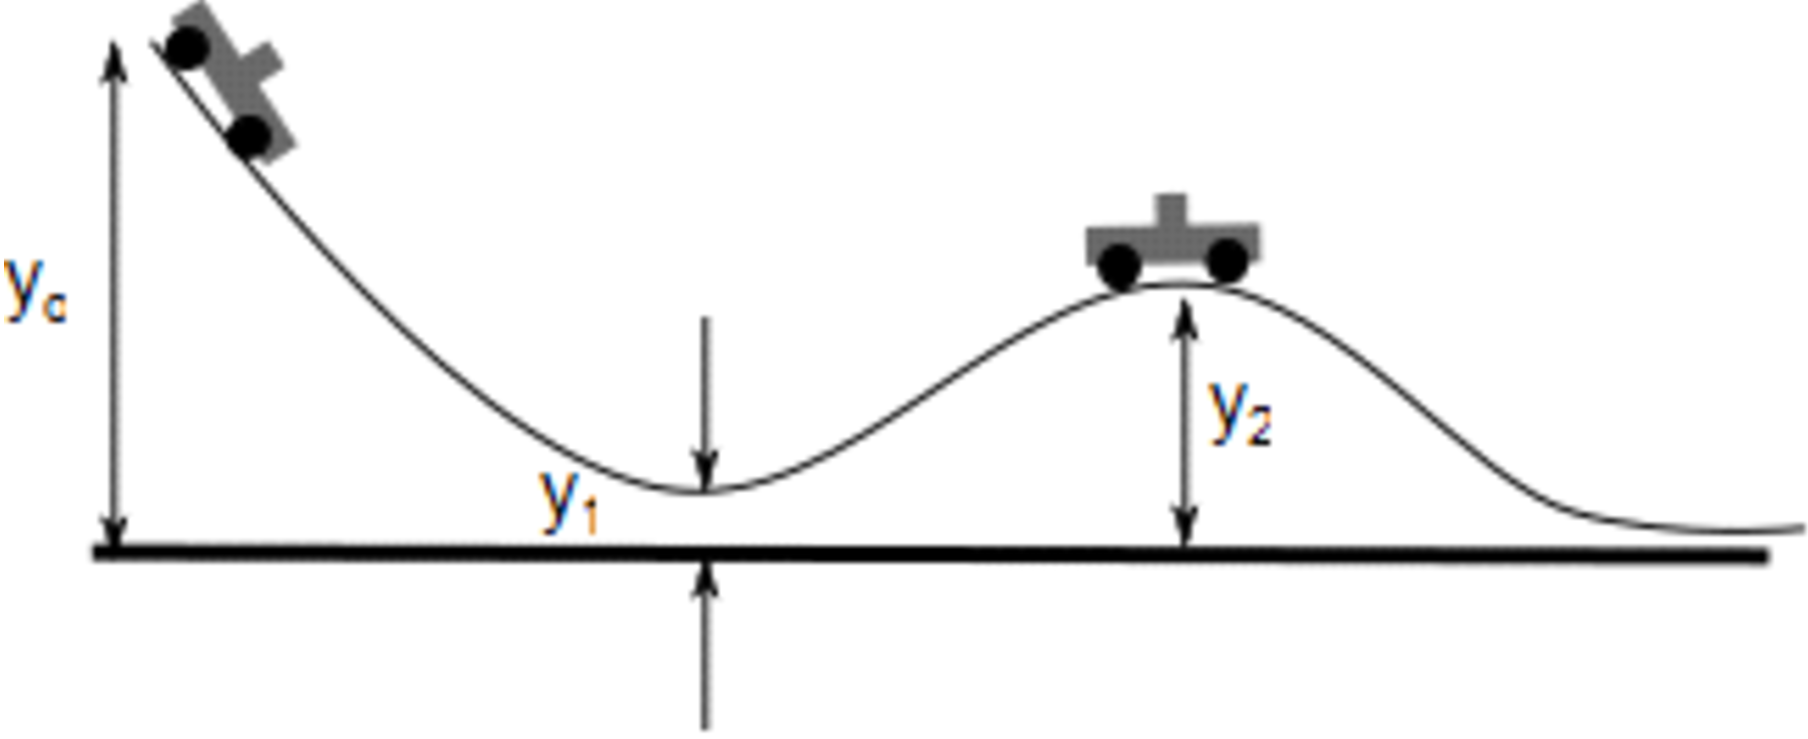
\includegraphics[width=0.5\textwidth]{Lab5_figs/LHDZMM03.png}
\end{center}
Your colleague suggests to you
that if energy is conserved, you should be able to predict the velocity of
the car at points $y_{1}$ and $y_{2}.$

Another colleague steps in and suggests that you need to be concerned about
the energy tied up in the rotational kinetic energy of the wheels. You may
not have heard about this in your PH121 class yet. She says that is OK,
because you can do a quick fix. She suggests that you should include a
factor of about 10\% of the translation kinetic energy. That is, compute the
kinetic energy in this case as%
\[
K=\left( 1.1\right) \frac{1}{2}mv^{2} 
\]%
that should account for the wheel rotational kinetic energy.

\pagebreak

\section{Assignment}

\subsection{Part 1:}

As a group design an experiment to test the model. Your design should
include the steps from lab \ref{Experimental Design} (briefly repeated here)

\begin{enumerate}
\item Identify the system to be examined. Identify the inputs and outputs.
Describe your system in your lab notebook.

\item Identify the model to be tested. Express the model in terms of an
equation representing a prediction of the measurement you will make. Record
this in your lab notebook. (If you have not solved this problem in your
PH121 class yet, call me over and we will go through it together).

\item Plan how you will know if you are successful in your experiment. Plan
graphs or other reporting devices. Record this in your lab notebook. For
today's lab, I\ will provide photogates and the car and track. If you need
other equipment, ask.

\item Rectify your equation if needed. Record this in your lab notebook.

\item Choose ranges of the variables. Record this in your lab notebook.

\item Plan the experimental procedure. Record this in your lab notebook.

\item Perform the experiment. Record this in your lab notebook. Go through
all the steps of performing an experiment. End with a conclusion that
clearly states whether your experiment supported the model, falsified the
model, or, if neither was possible, try to explain why.
\end{enumerate}

\subsection{Part 2}

Work on your proposals. They are due in two weeks. Here are some tips on
writing your proposal:

\subsubsection{Proposal writing:}

A Proposal is a document that is intended to persuade someone (your
professor, funding agency, yourself, etc.) that you should be given the
resources and support to perform the experiment. For our class, the proposal
consists of the following parts:

\begin{enumerate}
\item Statement of the experimental problem

\item Procedures and anticipated difficulties

\item Proposed analysis and expected results

\item Preliminary List of equipment needed
\end{enumerate}

Note that most of the steps involved in planning an experiment are contained
in these for parts of the proposal. Each of the steps is explained in more
detail below.

\paragraph{\textbf{Statement of the experimental problem:}}

This is a physics class, so our experiment should be a physics experiment.
The job of an experimental physicist is to test physics models. So your
statement of the experimental problem should include what model you are
testing and a brief, high level, overview of what you plan to do to test
this model.

\paragraph{\textbf{Procedures and anticipated difficulties:}}

Hopefully, your reader will be so excited by the thought of you solving your
experimental problem that he or she will want to know the details of what
you plan to do. You should describe in some detail what you are planning. If
there are hard parts of the procedure, tell how you plan to get through
them. This is essentially steps 1-6 of our experimental design strategy.

\paragraph{\textbf{Proposed analysis and expected results:}}

You might think this is unfair, how are you supposed to know what analysis
will be needed and what the results should be until you take the data? But
really you both can, and should make a good plan for your data analysis and
figure out what your expected results should be before you start taking
data. After all, you have a model you are testing. You can encapsulate that
model into a predictive equation for your experiment. Then you can use that
predictive equation to obtain predicted results and uncertainties. Using
this, you can design your experimental apparatus by putting in the numbers
from your experimental design and seeing what the outcome should be. You can
see if there is a chance that your experiment will measure what you want
with the equipment you have (this is where our differential form of error
calculation comes in).

If you don't do this, you don't know what equipment you will need or how
sensitive that equipment needs to be. If you are trying to measure the size
of your text book, an odometer that only measures in whole miles may not be
the best choice of equipment. This might be obvious, but depending on how
well you need to measure your text book, a ruler may not work either. You
don't know until you have an estimate of the uncertainty. So to know what
you need, do the calculations in advance with your range of inputs as the
values you take for the prediction.

Of course this means you must include a predictive calculation of the
uncertainty. Uncertainty in your result is governed by the uncertainty
inherent in the measurements you will take. The uncertainty calculation
tells you what sensitivity you will need in your measurement devices. In our
text book case, you could see immediately that you need a different
apparatus than the odometer. You might also find our ruler to be problematic
depending on what precision you need.

I remember a time in my career when the US\ Naval Research Labs asked us to
build a microwave radiometer to measure the sea wind direction from space.
We spent some time and our predicted analysis and uncertainty said that it
would be a very expensive instrument to be able to successfully measure the
wind direction---it would take more money than they were offering. NRL
disagreed and built the device themselves at less cost, but to lesser
specifications with much greater uncertainties. Then they spent a billion
(yes, a billion with a \textquotedblleft b\textquotedblright ) dollars to
launch the device into space. The device was a total failure. The
uncertainty was so big that the data was totally useless. We want to find
out whether our experiment will work before we risk our grades (or a billion
dollars) on it. So we will do the prediction ahead of taking the data.

You should do all of this symbolically if you can, numerically if you must,
but almost never by hand giving single value results. Some measurements will
come back poorer than you anticipated, or some piece of equipment will be
unavailable. You don't want to have to redo all your calculations from
scratch each time this happens. For example, in the event of an equipment
problem, your analysis tells you if another piece of equipment is
sufficiently sensitive, or if you need to find an exact replacement. When I\
perform an analysis like this, I try for a symbolic equation for
uncertainty. I\ like to program these equations into Scientific Workplace,
or Maple, or SAGE, or MathCAD, or Mathmatica or whatever symbolic math
processor I\ have. Then, as actual measurements change, I\ instantly get new
predictions. In the absence of a symbolic package, a spreadsheet program
will do fine (and we have Excel on our computers). A numerical program also
is quick and easy to re-run with new numbers when no symbolic answer is
found.

\subsubsection{Preliminary List of equipment needed}

Once you have done your analysis, you are ready to list the equipment you
need and the sensitivity of the equipment you need (that is, list the
uncertainties you need to achieve). Final approval of the project and the
ultimate success of your experiment depends on the equipment you choose or
are granted. You want to do a good job analyzing so you know what you need,
and a good job describing the experiment so you are likely to have the
equipment you want available when you start.

\subsubsection{Performing the experiment}

Once your proposal is accepted, I\ will provide you with the equipment we
have agreed upon from your proposal. You will have three weeks to perform
your experimentation. I\ will be available for advice and to watch for
problems or safety issues. But you and your team will perform the
experiment. \textbf{You will want to keep good notes in your lab notebook.}
You will likely have to change your procedure after you start because of
problems. Take careful note of what was actually done, and what your
measurements were. Give the reason for the change. Note any unusual things
that happen. \textbf{Carefully record what you do.}

\subsubsection{Written report}

The written report is designed to match a normal format for an applied
physics article in a journal like \emph{Applied Optics} or the \emph{IEEE
Transactions} journals.\emph{\ }It is useful to know now how I\ will grade
the report later so you can make sure you design in all the parts I will
look for. There should be an introduction, description of the procedure,
description of the data and results, a description of the analysis, and a
conclusion. These sections are described in detail in the following table.

Experimentation is a lot of fun if done right. It can be frustrating and
discouraging if not done well. Our goal is to learn how to perform and
report on an experiment, so that is what will be graded. If you show
something new and interesting, that is just more fun. If you show that your
original model was not correct--that is science! If you have done a good job
designing and reporting your experiment, a negative result is just as good
as a positive result.




\end{document}